\documentclass[12pt]{article}

\usepackage{bm}
\usepackage{amsmath}
\usepackage{amsfonts}
\usepackage{amssymb}
\usepackage{graphicx}
\usepackage{colortbl}
\usepackage{xr}
\usepackage{hyperref}
\usepackage{longtable}
\usepackage{xfrac}
\usepackage{tabularx}
\usepackage{float}
\usepackage{siunitx}
\usepackage{booktabs}

%\usepackage{refcheck}
\usepackage{graphicx}

\hypersetup{
    bookmarks=true,         % show bookmarks bar?
      colorlinks=true,       % false: boxed links; true: colored links
    linkcolor=red,          % color of internal links (change box color with linkbordercolor)
    citecolor=green,        % color of links to bibliography
    filecolor=magenta,      % color of file links
    urlcolor=cyan           % color of external links
}

\usepackage{fullpage}

\begin{document}

\title{Test Report} 
\author{Alex Guerrero, Keyur Patel and Shafeeq Rabbani}
\date{\today}

\maketitle

\section{Revisions}
\begin{center}
	\begin{longtable}{ | r | p{4cm} | p{4cm} | p{4cm} |}
	\caption{Revisions} \\ \hline \label{TblInputVar} 
	Name & Date & Description\\ \hline
	Keyur Patel & 27/11/2015 &  Created Test Report latex file\\ \hline
<<<<<<< HEAD
	Keyur Patel & 27/11/2015 &  Added table template for unit testing AND info\\ \hline
=======
	Alex Guerrero & 27/11/2015 & Edited Structural Testing\\ \hline
	\end{longtable}
\end{center}

\section{Structural (White Box) Testing}

\subsection{Unit Tests for Food}

\begin{center}
	\begin{longtable}{ | p{3cm} | p{4cm} | p{4cm} | p{2cm} |}
	\caption{Revisions} \\ \hline \label{TblInputVar} 
	Test Case & Initial State & Expected Output & Output\\ \hline
	testRandomPos.1 & foodA and foodB randomly placed & positions compared and not equal & pass  \\ \hline
	testRandomPos.2 & foodC randomly placed & || & pass  \\ \hline
	testRandomPos.3 & foodD randomly placed & || & pass  \\ \hline
>>>>>>> 5999134f4920b5ddc8bf8bfe8614070f6cb1bf9b
	\end{longtable}
\end{center}

\tableofcontents
\newpage



\section{Features that were Tested}

\begin{itemize}
\item 1:The functional requirements of the product
\item 2:The classes and methods of the product (Model)
\item 3:The GUI of the product
\end{itemize}

\section{Testing Types}
Testing can be broken up into different types, which each have their own role in the testing the product. These test types should be utilized to comprehensively evaluate the quality of the product.
\subsection{Structural Testing}
Structural testing  is also known as white box testing. Structural tests are derived from the program's internal structure. It focuses on the nonfunctional requirements of the product. This type of testing shows errors that occur during the implementation by focusing on abnormal and extreme cases the product could encounter.
\subsection{Functional Testing}
Functional testing is also known as black box testing. Functional tests are derived from the functional requirements of the program. It focuses less on how the program works and more on the output of the system. These tests are focused on test cases where the product receives expected information.
\subsection{Static vs. Dynamic Testing}
Static testing simulate the dynamic environment and does not focus on code exectution. This testing involves code walkthroughs and requirements walkthroughs. Static testing is used prevalently in the design stage. In contrast, dynamic testing needs code to be executed. \newline\newline
Dynamic testing involves test cases to be run and checked against expected outcomes. A technique to save time during dynamic testing is to choose representative test cases. 
\subsection{Manual vs. Automatic Testing}
Manual testing is done by people. It involves code walkthroughs and inspection. \newline\newline
Automatic testing can usually be conducted by computers. The tools used to assist with automatic are unit testing tools for the respective programming language. Automatic testing relies on people for testing more qualitative aspects like GUI. 


\section{Automated Unit Testing}
\subsection{Testing for Snake.py}
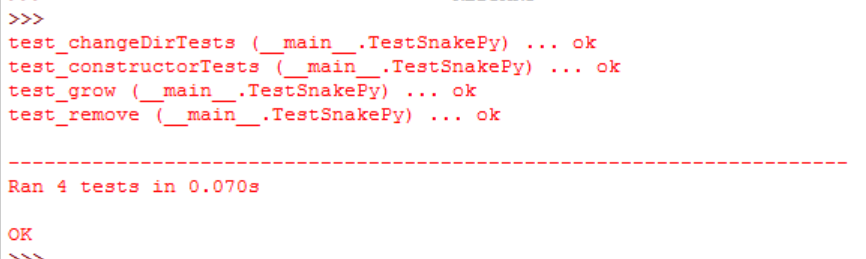
\includegraphics{testSnakeResults}\newline\newline
\begin{center}
	\begin{longtable}{ | r | p{4cm} | p{10cm} }
	\caption{Test Case for constructor} \\ \hline \label{TblInputVar} 
	\textbf{Function Tested} & Snake()\\ \hline
	\textbf{Preconditions} & none \\ \hline
	\textbf{Expected outcome} & a Snake() object is instantiated \\ \hline
	\textbf{Function Input} & none \\ \hline
	\textbf{Test Description} & This test asserts equality of two Snake() objects once in\\ \hline
	\textbf{Testing Type} & Correctness\\ \hline
	
	\end{longtable}
\end{center}

\begin{center}
	\begin{longtable}{ | r | p{4cm} | p{10cm} }
	\caption{Test Case for changeDir} \\ \hline \label{TblInputVar} 
	\textbf{Function Tested} & changeDir(newDirection)\\ \hline
	\textbf{Preconditions} & Snake object is already instantiated \\ \hline
	\textbf{Expected outcome} & The test object's direction is updated if it is a valid input \\ \hline
	\textbf{Function Input} & an integer from [-1,1,-2,2] \\ \hline
	\textbf{Test Description} & This test uses Snake objects in different directions and calls changeDir on them with all possible direciton inputs\\ \hline
	\textbf{Testing Type} & Correctness and Robustness\\ \hline
	
	\end{longtable}
\end{center}

\begin{center}
	\begin{longtable}{ | r | p{4cm} | p{10cm} }
	\caption{Test Case for grow} \\ \hline \label{TblInputVar} 
	\textbf{Function Tested} & grow\\ \hline
	\textbf{Preconditions} & there is an instantiated Snake() object \\ \hline
	\textbf{Expected outcome} & The snake's length increases by 1 \\ \hline
	\textbf{Function Input} & none \\ \hline
	\textbf{Test Description} & This test asserts equality between pregrown Snake objects and newly grown objects\\ \hline
	\textbf{Testing Type} & Correctness\\ \hline
	
	\end{longtable}
\end{center}

\begin{center}
	\begin{longtable}{ | r | p{4cm} | p{10cm} }
	\caption{Test Case for remove} \\ \hline \label{TblInputVar} 
	\textbf{Function Tested} & remove\\ \hline
	\textbf{Preconditions} & a Snake object is instantiated \\ \hline
	\textbf{Expected outcome} & every point in the snake after the inputted index is removed \\ \hline
	\textbf{Function Input} & integer value corresponding to the index \\ \hline
	\textbf{Test Description} & This test asserts equality between the length of a Snake object that has remove executed at various indexes and said indexes+1. This test also tests for abnormal and extreme values\\ \hline
	\textbf{Testing Type} & Correctness,Robustness\\ \hline
	
	\end{longtable}
\end{center}

\subsection{Testing for MainMenu.py}
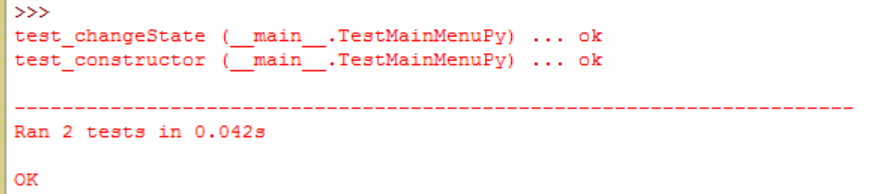
\includegraphics{testMainMenuResults}\newline\newline
\begin{center}
	\begin{longtable}{ | r | p{4cm} | p{10cm} }
	\caption{Test Case for constructor} \\ \hline \label{TblInputVar} 
	\textbf{Function Tested} & MainMenu() \\ \hline
	\textbf{Preconditions} & none \\ \hline
	\textbf{Expected outcome} & a MainMenu object is instantiated \\ \hline
	\textbf{Function Input} & none \\ \hline
	\textbf{Test Description} & constructor equality test\\ \hline
	\textbf{Testing Type} & Correctness\\ \hline
	
	\end{longtable}
\end{center}

\begin{center}
	\begin{longtable}{ | r | p{4cm} | p{10cm} }
	\caption{Test Case for changeState} \\ \hline \label{TblInputVar} 
	\textbf{Function Tested} & changeState\\ \hline
	\textbf{Preconditions} & a MainMenu object has been instantiated \\ \hline
	\textbf{Expected outcome} & the state is updated if input is valid \\ \hline
	\textbf{Function Input} & string value corresponding to the new state \\ \hline
	\textbf{Test Description} & This test asserts equality between the inputted newState and the state of the MainMenu object after running changeState on it\\ \hline
	\textbf{Testing Type} & Correctness,Robustness\\ \hline
	
	\end{longtable}
\end{center}


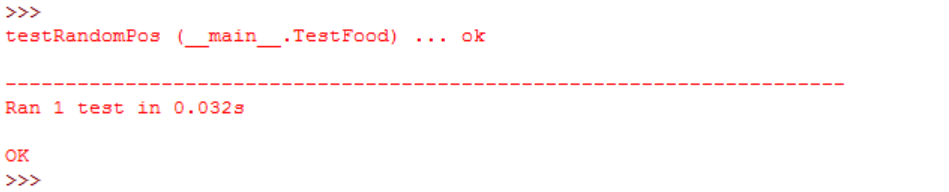
\includegraphics{testFoodResults}\newline\newline

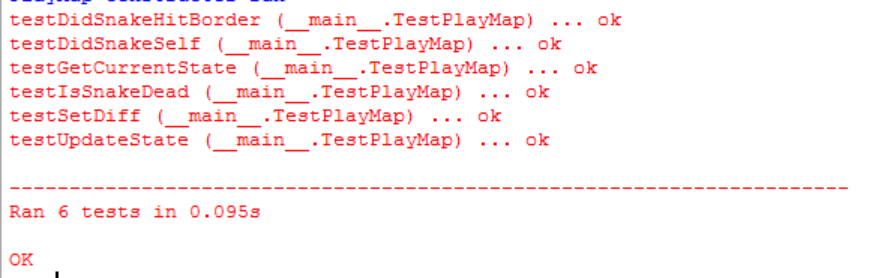
\includegraphics{testPlayMapResults}\newline\newline
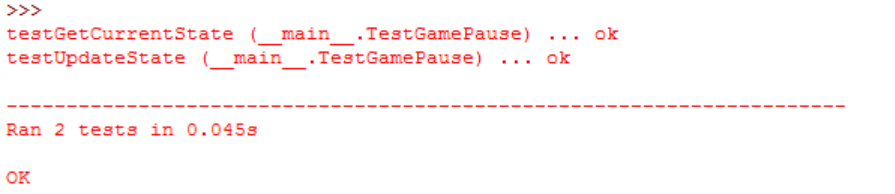
\includegraphics{testGamePauseResults}\newline\newline
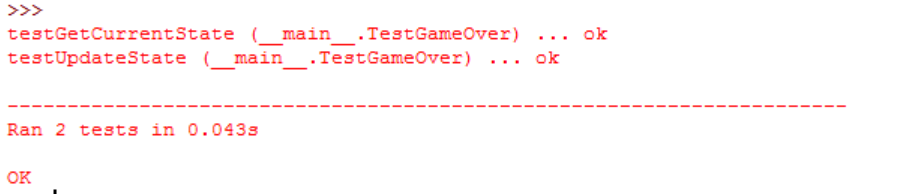
\includegraphics{testGameOverResults}\newline\newline

\section{Testing functional requirements}

\end{document}
